\documentclass{beamer}
\usetheme{Boadilla}        % Clean and modern theme
\usecolortheme{dolphin}    % Subtle blue-gray accent
\usepackage{graphicx}      % For including images
\usepackage{amsmath}       % For math symbols
\usepackage{hyperref}      % For clickable links

% Metadata
\title[Intro to LaTeX]{Introduction to LaTeX}
\subtitle{Beginner's Workshop with Code and Output}
\author{Prof. Shiburaj P.}
\institute[RCOE]{Rizvi College of Engineering}
\date{\today}

\begin{document}

% Title Slide
\begin{frame}
  \titlepage
\end{frame}

% Outline
\begin{frame}{Outline}
  \tableofcontents
\end{frame}

% Section 1: What is LaTeX
\section{What is LaTeX?}
\begin{frame}{Why LaTeX?}
\begin{itemize}
    \item High-quality typesetting system
    \item Widely used in scientific and academic writing
    \item Ideal for:
      \begin{itemize}
          \item Mathematical equations
          \item Figures and tables
          \item References and citations
      \end{itemize}
    \item Open-source and portable
\end{itemize}
\end{frame}

% Section 2: Document Structure
\section{Document Structure}
\begin{frame}[fragile]{Basic Document Structure}
\textbf{Code:}
\begin{verbatim}
\documentclass{report}

\begin{document}
Hello, world!
\end{document}
\end{verbatim}

\vspace{0.5cm}

\textbf{Output:}

Hello, world!
\end{frame}

% Section 3: Text Formatting
\section{Text Formatting}
\begin{frame}[fragile]{Text Formatting Example}
\textbf{Code:}
\begin{verbatim}
\textbf{Bold Text}
\textit{Italic Text}
\underline{Underlined Text}
\end{verbatim}

\vspace{0.5cm}

\textbf{Output:}

\textbf{Bold Text} \\
\textit{Italic Text} \\
\underline{Underlined Text}
\end{frame}


\begin{frame}[fragile]{Line Breaks Example}
\textbf{Code:}
\begin{verbatim}
This is line one. \\
This is line two. \\[0.5cm]
This is line three.
\end{verbatim}

\vspace{0.5cm}

\textbf{Output:}

This is line one. \\
This is line two. \\[0.5cm]
This is line three.
\end{frame}

\begin{frame}[fragile]{Paragraphs Example}
\textbf{Code:}
\begin{verbatim}
This is the first paragraph.

This is the second paragraph.
\end{verbatim}

\vspace{0.5cm}

\textbf{Output:}

This is the first paragraph.

This is the second paragraph.
\end{frame}


% Lists Example
\begin{frame}[fragile]{Lists Example : itemize}
\textbf{Code:}
\begin{verbatim}
\begin{itemize}
    \item First item
    \item Second item
\end{itemize}

\end{verbatim}

\vspace{0.5cm}

\textbf{Output:}

\begin{itemize}
    \item First item
    \item Second item
\end{itemize}

\end{frame}

\begin{frame}[fragile]{Lists Example : enumerate}
\textbf{Code:}
\begin{verbatim}

\begin{enumerate}
    \item First item
    \item Second item
\end{enumerate}
\end{verbatim}

\vspace{0.5cm}

\textbf{Output:}

\begin{enumerate}
    \item First item
    \item Second item
\end{enumerate}
\end{frame}

\section{Text Alignment}

\begin{frame}[fragile]{Center Alignment}
\textbf{Code:}
\begin{verbatim}
\begin{center}
This text is centered.
\end{center}
\end{verbatim}

\vspace{0.5cm}

\textbf{Output:}

\begin{center}
This text is centered.
\end{center}
\end{frame}

\begin{frame}[fragile]{Left and Right Alignment}
\textbf{Code:}
\begin{verbatim}
\begin{flushleft}
This text is left aligned.
\end{flushleft}

\begin{flushright}
This text is right aligned.
\end{flushright}
\end{verbatim}

\vspace{0.5cm}

\textbf{Output:}

\begin{flushleft}
This text is left aligned.
\end{flushleft}

\begin{flushright}
This text is right aligned.
\end{flushright}
\end{frame}

\begin{frame}[fragile]{Justified Text}
\textbf{Code:}
\begin{verbatim}
\begin{justify}
This text is justified. 
It spreads across the full width.
\end{justify}
\end{verbatim}

\vspace{0.5cm}

\textbf{Output:}

\begin{flushleft} % fallback since justify env needs extra pkg
This text is justified. 
It spreads across the full width.
\end{flushleft}
\end{frame}

% Section: Fonts and Sizes
\section{Fonts and Sizes}

\begin{frame}[fragile]{Changing Font Sizes}
\begin{columns}
\column{0.5\textwidth}
\textbf{Code:}
\begin{verbatim}
{\tiny Tiny Text}
{\scriptsize Script Size}
{\footnotesize Footnote Size}
{\small Small Text}
{\normalsize Normal Text}
{\large Large Text}
{\Large Larger Text}
{\LARGE Even Larger Text}
{\huge Huge Text}
{\Huge Biggest Text}
\end{verbatim}

\column{0.5\textwidth}
\textbf{Output:}

{\tiny Tiny Text} \\
{\scriptsize Script Size} \\
{\footnotesize Footnote Size} \\
{\small Small Text} \\
{\normalsize Normal Text} \\
{\large Large Text} \\
{\Large Larger Text} \\
{\LARGE Even Larger Text} \\
{\huge Huge Text} \\
{\Huge Biggest Text}
\end{columns}
\end{frame}

\begin{frame}[fragile]{Different Font Families}
\textbf{Code:}
\begin{verbatim}
\textrm{Roman Family} 

\textsf{Sans Serif Family}

\texttt{Typewriter Family}
\end{verbatim}

\vspace{0.5cm}

\textbf{Output:}

\textrm{Roman Family} \\
\textsf{Sans Serif Family} \\
\texttt{Typewriter Family}

\end{frame}


\section{Mathematics}

\begin{frame}[fragile]{Inline vs Block Math}
\textbf{Code:}
\begin{verbatim}
Inline math: $E = mc^2$

Block math:
\[
a^2 + b^2 = c^2
\]
\end{verbatim}

\vspace{0.5cm}

\textbf{Output:}

Inline math: $E = mc^2$

Block math:
\[
a^2 + b^2 = c^2
\]
\end{frame}

\begin{frame}[fragile]{Numbered Equations}
\textbf{Code:}
\begin{verbatim}
\begin{equation}
F = G \frac{m_1 m_2}{r^2}
\end{equation}
\end{verbatim}

\vspace{0.5cm}

\textbf{Output:}

\begin{equation}
F = G \frac{m_1 m_2}{r^2}
\end{equation}
\end{frame}

\begin{frame}[fragile]{Labeling and Referring Equations}
\textbf{Code:}
\begin{verbatim}
\begin{equation}
E = mc^2 \label{eq:einstein}
\end{equation}

As seen in equation~\ref{eq:einstein}, 
energy and mass are related.
\end{verbatim}

\vspace{0.5cm}

\textbf{Output:}

\begin{equation}
E = mc^2 \label{eq:einstein}
\end{equation}

As seen in equation~\ref{eq:einstein}, 
energy and mass are related.
\end{frame}

\begin{frame}{Online Tools to Make Latex Equations}

\begin{itemize}
    \item \textbf{Site 1} : \url{https://editor.codecogs.com/}
    \item \textbf{Site 2} : \url{https://latexeditor.lagrida.com/}
    \item \textbf{Site 3} : Use Overleaf Equation Generator or ChatGPT
\end{itemize}

\end{frame}

% Section: Tables
\section{Tables}

\begin{frame}[fragile]{Simple Table}
\textbf{Code:}
\begin{verbatim}
\begin{tabular}{c c}
A & B \\
C & D
\end{tabular}
\end{verbatim}

\vspace{0.5cm}

\textbf{Output:}

\begin{tabular}{c c}
A & B \\
C & D
\end{tabular}
\end{frame}

\begin{frame}[fragile]{Table with Borders}
\textbf{Code:}
\begin{verbatim}
\begin{tabular}{|c|c|}
\hline
Name & Score \\
\hline
Alice & 95 \\
Bob & 88 \\
\hline
\end{tabular}
\end{verbatim}

\vspace{0.5cm}

\textbf{Output:}

\begin{tabular}{|c|c|}
\hline
Name & Score \\
\hline
Alice & 95 \\
Bob & 88 \\
\hline
\end{tabular}
\end{frame}

\begin{frame}[fragile]{Table with Caption and Label}
\begin{columns}
\column{0.5\textwidth}
\textbf{Code:}
\begin{verbatim}
\begin{table}
\centering
\begin{tabular}{|c|c|}
\hline
Country & Capital \\
\hline
India & New Delhi \\
USA & Washington DC \\
\hline
\end{tabular}
\caption{List of Countries}
\label{tab:countries}
\end{table}

See Table~\ref{tab:countries} for details.
\end{verbatim}

\column{0.5\textwidth}

\textbf{Output:}

\begin{table}
\centering
\begin{tabular}{|c|c|}
\hline
Country & Capital \\
\hline
India & New Delhi \\
USA & Washington DC \\
\hline
\end{tabular}
\caption{List of Countries}
\label{tab:countries}
\end{table}
See Table~\ref{tab:countries} for details.
\end{columns}

\end{frame}

\begin{frame}[fragile]{Online Tools to Make Tables}

\begin{itemize}
    \item \textbf{Site 1} : \url{https://www.tablesgenerator.com/#}
    \item \textbf{Site 2} : \url{https://www.latex-tables.com/}
    \item \textbf{Site 3} : Use Overleaf Table Generator or ChatGPT
\end{itemize}

\end{frame}

% Section: Figures
\section{Figures}

\begin{frame}[fragile]{Including a Simple Image}
\textbf{Code:}
\begin{verbatim}

\includegraphics{rcoe-logo.png}
\end{verbatim}

\vspace{0.5cm}

\textbf{Output:}


\includegraphics{rcoe-logo.png}    

\end{frame}

\begin{frame}[fragile]{Resizing an Image}
\textbf{Code:}
\begin{verbatim}

\includegraphics[width=0.5\textwidth]{rcoe-logo.png}
\end{verbatim}

\vspace{0.5cm}

\textbf{Output:}


\includegraphics[width=0.5\textwidth]{rcoe-logo.png}
\end{frame}

\begin{frame}[fragile]{Image with Caption and Label}
\textbf{Code:}
\begin{verbatim}
\begin{figure}
\centering

\includegraphics[width=0.2\textwidth]{rcoe-logo.png}
\caption{Sample Figure}
\label{fig:sample}
\end{figure}

As shown in Figure~\ref{fig:sample}, 
this is an example image.
\end{verbatim}
\end{frame}

\begin{frame}{Image with Caption and Label: Output}
    
\textbf{Output:}

\begin{figure}
\centering

\includegraphics[width=0.2\textwidth]{rcoe-logo.png}
\caption{Sample Figure}
\label{fig:sample}
\end{figure}

As shown in Figure~\ref{fig:sample}, 
this is an example image.
\end{frame}

% Section: Citations and References
\section{Citations and References}

\begin{frame}[fragile]{Adding a Citation}
\textbf{Code:}
\begin{verbatim}
According to \cite{einstein}, 
energy and mass are related.
\end{verbatim}

\vspace{0.5cm}

\textbf{Output:}

According to \cite{einstein}, energy and mass are related.
\end{frame}

\begin{frame}[fragile]{Creating a .bib File}
\textbf{Code in refs.bib:}
\begin{verbatim}
@article{einstein,
  author  = {Albert Einstein},
  title   = {Does the Inertia of a Body Depend Upon Its Energy Content?},
  journal = {Annalen der Physik},
  year    = {1905},
}
\end{verbatim}

\textbf{Code in main.tex:}
\begin{verbatim}
\bibliographystyle{plain}
\bibliography{refs}
\end{verbatim}
\end{frame}

\begin{frame}[fragile]{Output of References}
\textbf{Output:}

According to \cite{einstein}, energy and mass are related.

\vspace{0.5cm}

\textbf{References:}
\begin{thebibliography}{9}
\bibitem{einstein}
Albert Einstein.
\newblock Does the Inertia of a Body Depend Upon Its Energy Content?
\newblock {\em Annalen der Physik}, 1905.
\end{thebibliography}
\end{frame}

% Summary Slide
\begin{frame}{Summary}
\begin{itemize}
    \item LaTeX is a powerful tool for professional documents
    \item Topics covered:
      \begin{itemize}
          \item Document structure
          \item Text formatting and lists
          \item Mathematical equations
          \item Tables and figures
          \item References
      \end{itemize}
    \item Practice is key!
\end{itemize}
\end{frame}

%----------------------------------------
% Hands-on Exercise: Resume
%----------------------------------------
\section{Exercise}

\begin{frame}[fragile]{Hands-on Exercise: Build Your Resume}
\textbf{Task:} Create a one-page resume using \LaTeX.

\bigskip
\textbf{Include the following:}
\begin{itemize}
    \item \textbf{Name} in large bold font
    \item \textbf{Tagline} (e.g., *"Student | Developer"*)
    \item \textbf{Photo} (insert with \verb|\includegraphics|)
    \item \textbf{Short Bio} (3–4 lines)
    \item \textbf{Education} (table or list with degree, year, institution)
    \item \textbf{Projects} (at least 2 with short description)
    \item \textbf{Skills} (list 5–6 skills)
\end{itemize}

\bigskip
\textbf{Bonus:} Use alignment, colors, and formatting to make it professional.
\end{frame}

\begin{frame}{Sample}
    \begin{center}
        {\Huge \textbf{Shiburaj Pappu}} \\
        {\large \textit{Dean of Academics}} \\[0.1cm]
        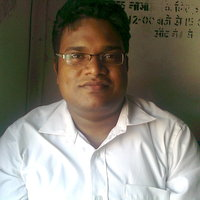
\includegraphics[width=3cm]{photo.jpg}
    \end{center}
    
    \section*{Bio}
    A post graduate in Engineering from Mumbai University, Prof. Shiburaj P. is passionate about innovation \& research. For him his work is of prime importance.
    
    \section*{Education}
    - Degree, Year, Institution
    
    \section*{Projects}
    - Project 1: Description
    - Project 2: Description
    
    \section*{Skills}
    Skill1, Skill2, Skill3
\end{frame}

% Questions Slide
\begin{frame}
  \centering
  {\Huge Questions?}
\end{frame}

\begin{frame}
  \begin{columns}
      \column{0.5\textwidth}
      \begin{figure}
          \centering
          
\includegraphics[width=0.5\linewidth]{synopsis.png}
      \end{figure}
      \centering
      \href{https://github.com/shiburaj/latex-synopsis-report}{Synopsis Report Template}
      \column{0.5\textwidth}
      \begin{figure}
          \centering
          
\includegraphics[width=0.5\linewidth]{project.png}
      \end{figure}
      \centering
      \href{https://github.com/shiburaj/latex-project-report}{Project Report Template}
  \end{columns}
\end{frame}

\end{document}
